\documentclass{sigchi}

% Use this section to set the ACM copyright statement (e.g. for
% preprints).  Consult the conference website for the camera-ready
% copyright statement.

% Copyright
\CopyrightYear{2017}
% \setcopyright{acmcopyright}
% \setcopyright{acmlicensed}
\setcopyright{rightsretained}
%\setcopyright{usgov}
%\setcopyright{usgovmixed}
%\setcopyright{cagov}
%\setcopyright{cagovmixed}

% % DOI
% \doi{http://dx.doi.org/10.475/123_4}
%
% % ISBN
% \isbn{123-4567-24-567/08/06}

%Conference
\conferenceinfo{Thirty-three Month Report,}{20 May 2017, Birmingham, UK}

%Price
% \acmPrice{\$XX.00}

% Use this command to override the default ACM copyright statement
% (e.g. for preprints).  Consult the conference website for the
% camera-ready copyright statement.

%% HOW TO OVERRIDE THE DEFAULT COPYRIGHT STRIP --
%% Please note you need to make sure the copy for your specific
%% license is used here!
% \toappear{
% Permission to make digital or hard copies of all or part of this work
% for personal or classroom use is granted without fee provided that
% copies are not made or distributed for profit or commercial advantage
% and that copies bear this notice and the full citation on the first
% page. Copyrights for components of this work owned by others than ACM
% must be honored. Abstracting with credit is permitted. To copy
% otherwise, or republish, to post on servers or to redistribute to
% lists, requires prior specific permission and/or a fee. Request
% permissions from \href{mailto:Permissions@acm.org}{Permissions@acm.org}. \\
% \emph{CHI '16},  May 07--12, 2016, San Jose, CA, USA \\
% ACM xxx-x-xxxx-xxxx-x/xx/xx\ldots \$15.00 \\
% DOI: \url{http://dx.doi.org/xx.xxxx/xxxxxxx.xxxxxxx}
% }

% Arabic page numbers for submission.  Remove this line to eliminate
% page numbers for the camera ready copy
% \pagenumbering{arabic}

% Load basic packages
\usepackage{balance}       % to better equalize the last page
\usepackage{graphics}      % for EPS, load graphicx instead
\usepackage[T1]{fontenc}   % for umlauts and other diaeresis
\usepackage{txfonts}
\usepackage{mathptmx}
\usepackage[pdflang={en-US},pdftex]{hyperref}
\usepackage{color}
\usepackage{booktabs}
\usepackage{textcomp}

% Some optional stuff you might like/need.
\usepackage{microtype}        % Improved Tracking and Kerning
% \usepackage[all]{hypcap}    % Fixes bug in hyperref caption linking
\usepackage{ccicons}          % Cite your images correctly!
% \usepackage[utf8]{inputenc} % for a UTF8 editor only

% If you want to use todo notes, marginpars etc. during creation of
% your draft document, you have to enable the "chi_draft" option for
% the document class. To do this, change the very first line to:
% "\documentclass[chi_draft]{sigchi}". You can then place todo notes
% by using the "\todo{...}"  command. Make sure to disable the draft
% option again before submitting your final document.
\usepackage{todonotes}



\usepackage{caption,subcaption}
% https://tex.stackexchange.com/questions/83069/how-to-stack-two-subfigures-next-to-a-third-subfigure


% Paper metadata (use plain text, for PDF inclusion and later
% re-using, if desired).  Use \emtpyauthor when submitting for review
% so you remain anonymous.

% \def\plaintitle{Movement Variability: 33 Month Report}
% \def\plaintitle{Movement Variability in the context of Human-Robot Imitation}
% \def\plaintitle{Nonlinear Dynamic Invariants for Movement Variability in the context of Human-Humanoid Imitation}
% \def\plaintitle{Movement Variability in the context of Human-Humanoid Interaction: 33 Month Report}
% \def\plaintitle{Movement Variability in the context of Human-Humanoid Interaction}
\def\plaintitle{Automatic Classification of Movement Variability in Human-Humanoid Interaction}

\def\plainauthor{}

\def\emptyauthor{}

% \def\plainkeywords{Authors' choice; of terms; separated; by
%   semicolons; include commas, within terms only; required.}
\def\plainkeywords{Human-Robot Interaction; Wearable Inertial Sensors; State Space Reconstruction}

\def\plaingeneralterms{Documentation, Standardization}

% llt: Define a global style for URLs, rather that the default one
\makeatletter
\def\url@leostyle{%
  \@ifundefined{selectfont}{
    \def\UrlFont{\sf}
  }{
    \def\UrlFont{\small\bf\ttfamily}
  }}
\makeatother
\urlstyle{leo}

% To make various LaTeX processors do the right thing with page size.
\def\pprw{8.5in}
\def\pprh{11in}
\special{papersize=\pprw,\pprh}
\setlength{\paperwidth}{\pprw}
\setlength{\paperheight}{\pprh}
\setlength{\pdfpagewidth}{\pprw}
\setlength{\pdfpageheight}{\pprh}

% Make sure hyperref comes last of your loaded packages, to give it a
% fighting chance of not being over-written, since its job is to
% redefine many LaTeX commands.
\definecolor{linkColor}{RGB}{6,125,233}
\hypersetup{%
  pdftitle={\plaintitle},
% Use \plainauthor for final version.
%  pdfauthor={\plainauthor},
  pdfauthor={\emptyauthor},
  pdfkeywords={\plainkeywords},
  pdfdisplaydoctitle=true, % For Accessibility
  bookmarksnumbered,
  pdfstartview={FitH},
  colorlinks,
  citecolor=black,
  filecolor=black,
  linkcolor=black,
  urlcolor=linkColor,
  breaklinks=true,
  hypertexnames=false
}

% create a shortcut to typeset table headings
% \newcommand\tabhead[1]{\small\textbf{#1}}


%https://tex.stackexchange.com/questions/271627/shared-author-affiliation-in-acm-sig-proc
\def\sharedaffiliation{%
\end{tabular}
\begin{tabular}{c}}

% End of preamble. Here it comes the document.
\begin{document}

\title{\plaintitle}

\numberofauthors{3}
\author{%
    \alignauthor Miguel P. Xochicale\\
    \affaddr{Doctoral Researcher}\\
    \email{map479@bham.ac.uk}
%
    \alignauthor Chris Baber\\
    \affaddr{Lead Supervisor}\\
    \email{c.baber@bham.ac.uk}
%
    \alignauthor Martin J. Russell\\
    \affaddr{Co-supervisor}\\
    \email{m.j.russell@bham.ac.uk}
%
    \sharedaffiliation
    \affaddr{School of Electronic, Electrical and Systems Engineering}  \\
    \affaddr{University of Birmingham, UK}
}

\maketitle

\begin{abstract}
  UPDATED---\today.
\end{abstract}

% \category{H.5.m.}{Information Interfaces and Presentation
%   (e.g. HCI)}{Miscellaneous} \category{See
%   \url{http://acm.org/about/class/1998/} for the full list of ACM
%   classifiers. This section is required.}{}{}

% \keywords{\plainkeywords}

% \section{Introduction}

%%%%%%%%%%%%%%%%%%%%%%%%%%%%%%%%%%%%%%%%%%%%%%%%%%%%%%%%%%%%%%%%%%%%%%%%%%%%%%%%
\section{1 Contributions}

For the moment, my scientific outcomes are still far from either being
scientifically impactful or creating original contributions.
Nonetheless, I would like to note that I have presented
% insightful
some results in conferences for which I have refined my main research question
% which reads
as follows:
\begin{itemize}
 \item \textit{
 How the movement variability can be used as an automatic index
 of users' performance over the course of practice in
 Human-Humanoid Interactions?
}
\end{itemize}
With this in mind, I coducted three experiments which results were reported
in three conferences of acceptance rate of less than 50\%
\cite{MXochicale:WeRob16, MXochicale:PerDis16, MXochicale:HRI2017}.
From the reviews' comments of the submitted work, I have learnt
the following lessons which
are helping the work
% will be helpful for the work
to create original contributions to science
and to make significant value of knownledge:
 % which are important help to get partial answers.
% make significant value of knownledge.
 % for my PhD project.

\begin{description}
  \setlength{\itemsep}{0pt}
  \setlength{\parskip}{0pt}
  \item [(i)]Performance of data collection from a wider range of individuals
  (different gender, age and state of health); from additional inertial sensors
  attached to different parts of the body and
  from different levels of movement complexity.

  \item [(ii)] Give an intrinsic explanation of the state space reconstruction
  in which is described why the time-delay embedding is an appropriate technique
  to analyse human movement variability and why is important to compare
  different methodologies for dimensiality reduction.
% supported by the reasons   of why these are  for this research.

  \item [(iii)] Provide quantificable evidence on how the postprocessing techniques
  (e.g. low-pass filtering, smoothing data, and interpolation) for the inertial
  sensors is affecting the metric to quantify movement variability.
  % To which I hyphotesise that it is unknown how
  % % It is
  % the postprocessing techniques are affecting the quantification of the movement
  % variability.
  % % for which there is little evidence on how much these techniques can
  % %  to make a transferable and
  % % therefore realiable metric.

  \item [(iv)] Provide a further understanding of human movememnt variablity in
  sceneaiors of Human to Humanoid interaction and Group of Humans to Humanoid interaction.
  For which besides the analysis of arm movements, I believe that head pose estimation
  can lead me to create better metrics and provide relationships of movement
  variability between the complexity of arm movements and the level of attention
  per participant.
  % Therefore,
  % implementation of algorithms and tools are of need to quantify automatically
  % the movement variability using wearable inertial sensors
  % in the context of human-humanoid interaction.
\end{description}







% Example reference formatting for
% individual journal articles~\cite{ethics}, articles in conference
% proceedings~\cite{Klemmer:2002:WSC:503376.503378},
% books~\cite{Schwartz:1995:GBF}, theses~\cite{sutherland:sketchpad},
% book chapters~\cite{winner:politics}, an entire journal
% issue~\cite{kaye:puc},
% websites~\cite{acm_categories,cavender:writing},
% tweets~\cite{CHINOSAUR:venue}, patents~\cite{heilig:sensorama},
% games~\cite{supermetroid:snes}, and
% online videos~\cite{psy:gangnam} is given here.




%%%%%%%%%%%%%%%%%%%%%%%%%%%%%%%%%%%%%%%%%%%%%%%%%%%%%%%%%%%%%%%%%%%%%%%%%%%%%%%%
\section{2 Workplan}
% A detailed workplan up to and including submission date;
A detailed workplan for the third and four year of the PhD project is presented
in Fig~\ref{fig:workplan} where a list of submissions for reports, conferences,
journals and thesis requirements are given with its respectively submission date.

The initialism and acronyms in Fig~\ref{fig:workplan}(a) have the following meaning:
HRI2017 is the 12th anual conference in Human-Robot Interaction 2017;
IMMX2017 is the second forum of Innovation for Talented Mexicans 2017;
MXSymposiumUK2017 is the 15th Annual Symposium of Mexican Students in the UK 2017;
HRI2018 is the 13th annual conference in Human-Robot Interaction 2018;
% Human Movement Journal;
and HAI2017 which is the 5th annual conference in Human-Agent Interaction 2017.
For Fig~\ref{fig:workplan}(b),
J. of Social Robotics is the International Journal of Social Robotics,
HRI2018 is the 13th annual conference in Human-Robot Interaction 2018,
and
MXSymposiumUK2018 is the 16th Annual Symposium of Mexican Students in the UK 2018.


\begin{figure}
\centering
  \begin{subfigure}[b]{0.5\textwidth}
  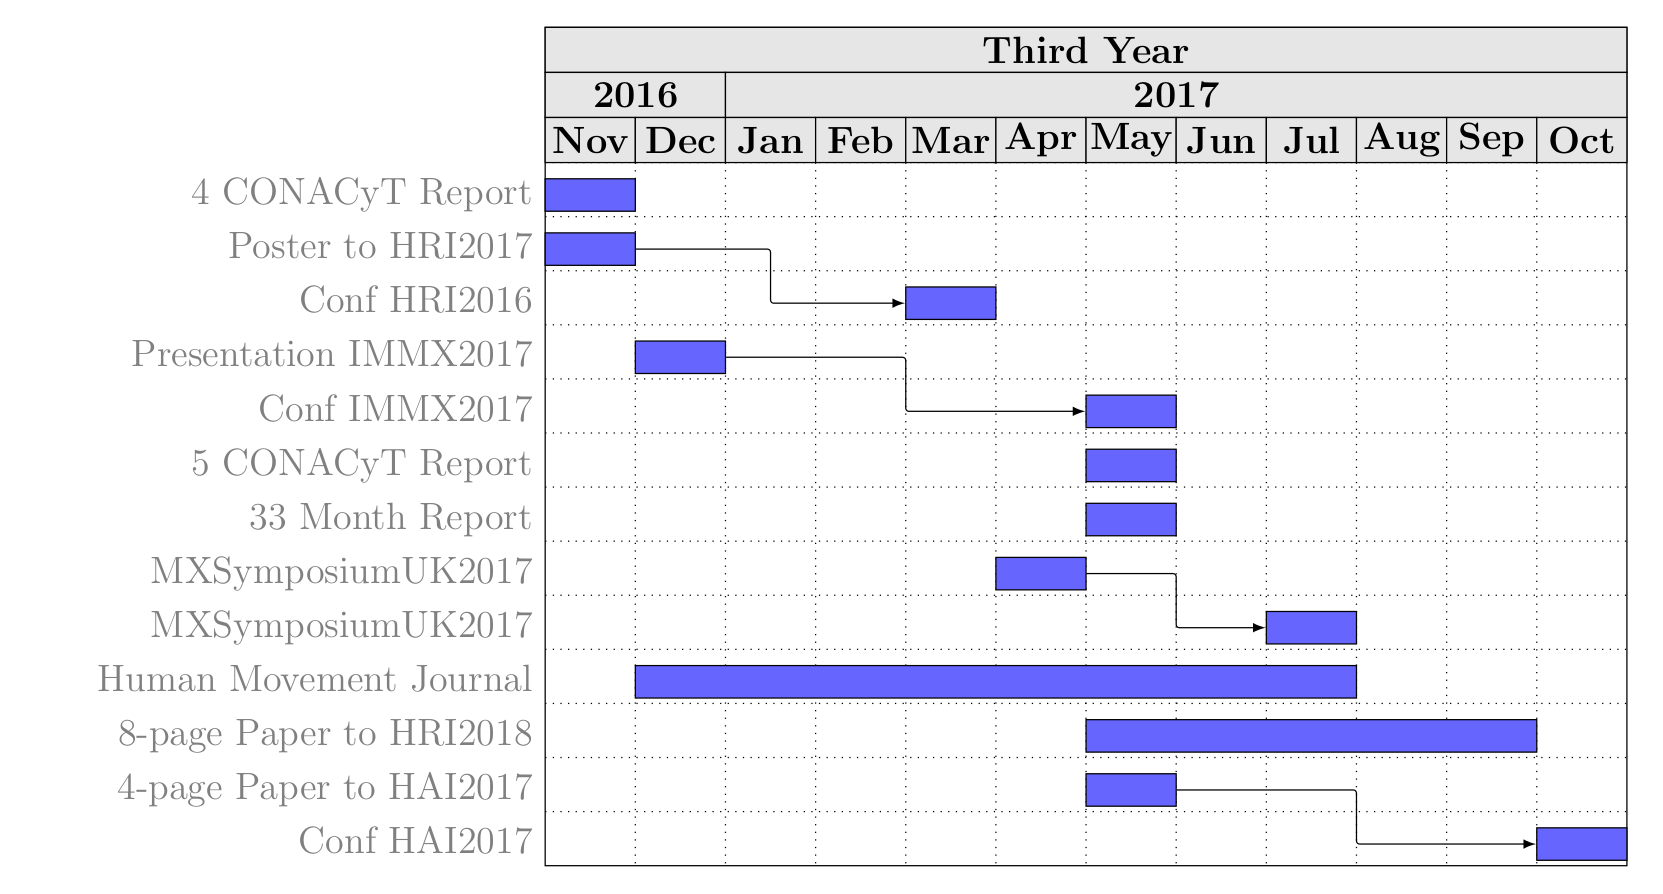
\includegraphics[width=0.9\columnwidth]{figures/third_year_b}
  \caption{Third year plan}
  \end{subfigure}\qquad

  \begin{subfigure}[b]{0.5\textwidth}
  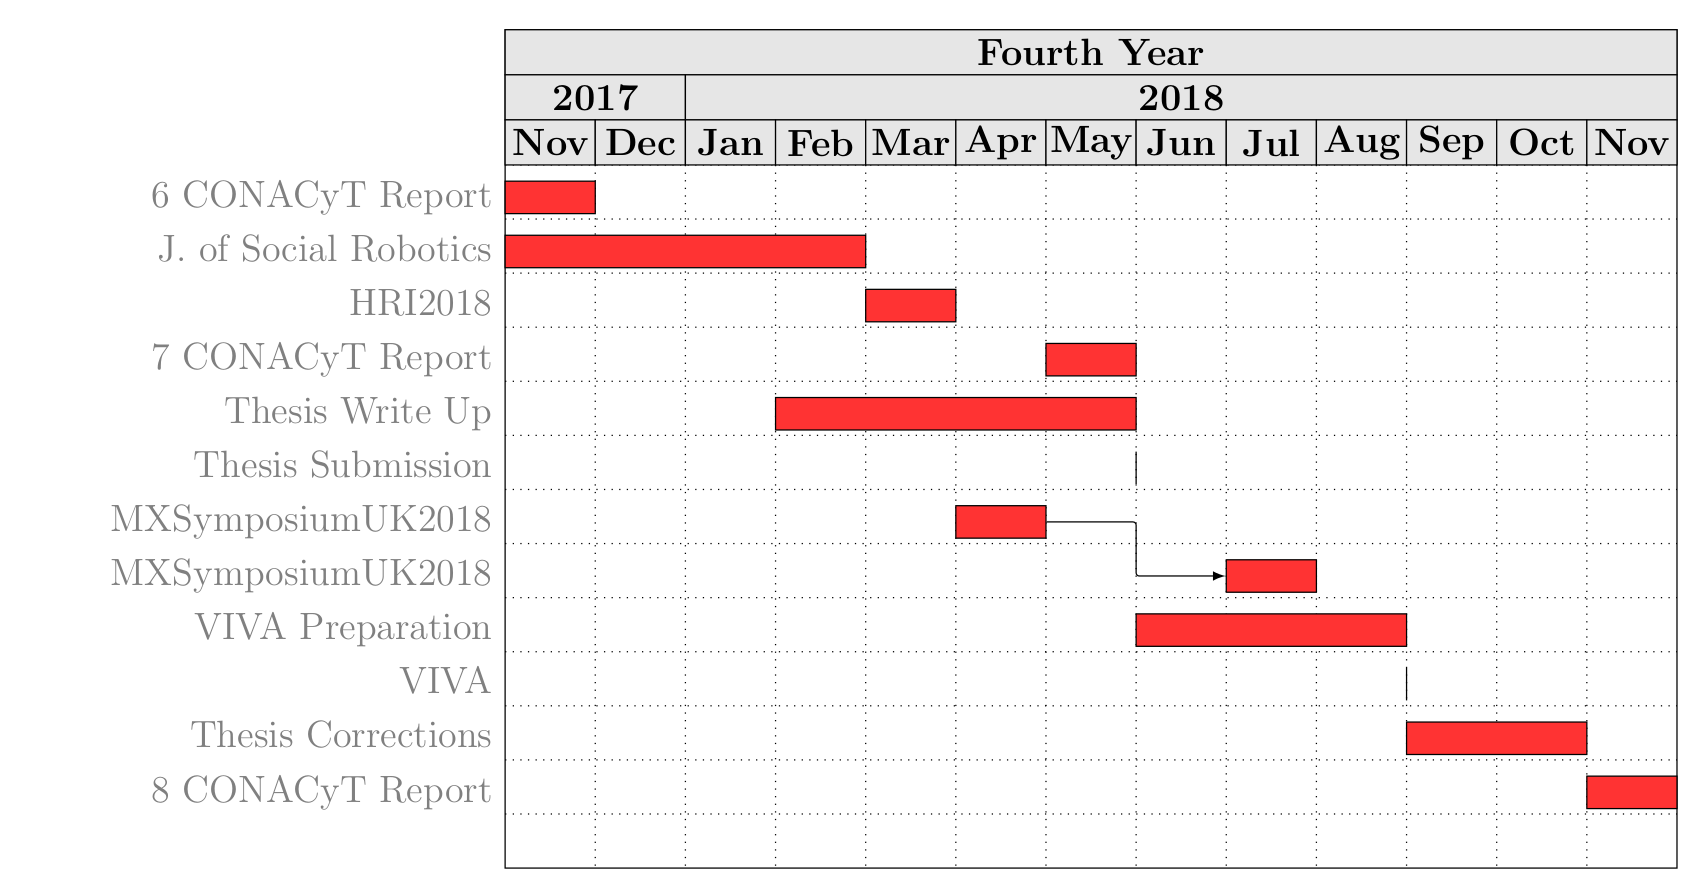
\includegraphics[width=0.9\columnwidth]{figures/fourth_year_b}
  \caption{Fourth year plan}
  \end{subfigure}\qquad

  \caption{Workplan}~\label{fig:workplan}
\end{figure}




%%%%%%%%%%%%%%%%%%%%%%%%%%%%%%%%%%%%%%%%%%%%%%%%%%%%%%%%%%%%%%%%%%%%%%%%%%%%%%%%
\section{3 Final Publication Plans}
I am planning to submit two conference papers and two manuscripts which
are described below:
\begin{itemize}
  \setlength{\itemsep}{0pt}
  \setlength{\parskip}{0pt}
  \item Submission of a 4-page paper to the 5th conference in Human-Agent
  Interaction which has an acceptance rate of 40\% to 50 \% (deadline: 2 June 2017 )
  \item Submission of a 8-page paper to the 13th anual conference in Human-Robot
  Interaction 2018 which has a rate of acceptance of 24\%. (deadline: 8 October 2017 )
  \item Manuscript submission to the Human Movement Journal which Impact Factor
  is 1.606 in 2015. (deadline: 31 July 2017)
  \item Manuscript submission to the International Journal of Social Robotics
  which Impact Factor is 1.407 in 2015. (deadline: 28 February 2018)
\end{itemize}









%%%%%%%%%%%%%%%%%%%%%%%%%%%%%%%%%%%%%%%%%%%%%%%%%%%%%%%%%%%%%%%%%%%%%%%%%%%%%%%%
\section{4 Thesis structure}
The completeness of the thesis is estimated to be at its 40\% to this month
(May 2017). The possible thesis structure including a list of chapters with
an estimated percentage of completeness and sections is described below:
\begin{description}
  \setlength{\itemsep}{0pt}
  \setlength{\parskip}{0pt}
\item[Chapter 1: Introduction  ......................................  (25\%)]
  Structure of the Introduction: Opening hook. Context.
  Gap in the literature. Reserach questions. Argument. Outline of logic.

\item[Chapter 2: Literature Review  .............................  (60\%) ]
  2.1 Sources of Variability in Human Movement.
  2.1.1. Sensors
  2.1.2. Variability within person and across persons
  2.1.3. Variability for simple and complex activities
  2.2 Techniques to measure human movement variability.

\item[Chapter 3: Methodology .....................................   (60\%)]
  3.1 Time-domain. 3.2 Frequency-domain. 3.3 Nonlinear dynamics domain.


\item[Chapter 4: Experiments  .....................................  (75\%)]
4.1 Dance. 4.2 Simple Movements. 4.3 Human-Humanoid Imitation.
4.4 Group Activity in Human-Humanoid Imitation.


\item[Chapter 5: Automatic Classification  ..................  (10\%)]
  5.1 Convolutional Neural Networks
  5.2 Convolutional Neural Networks Using time-series from Inertial Sensors.

\item[Chapter 6: Conclusions  ...........................................  (0\%)]
% \item[Apendix: Data collection with Wearable Inertial Sensors]
\end{description}




%%%%%%%%%%%%%%%%%%%%%%%%%%%%%%%%%%%%%%%%%%%%%%%%%%%%%%%%%%%%%%%%%%%%%%%%%%%%%%%%
\section{5 Viva Preparation}
As shown in Fig~\ref{fig:workplan}(b), the VIVA preparations are planning
to be done between June 2018 to August 2018 so as to present the VIVA
in the first week of September 2018.




% \section{Figures/Captions}
%
% Place figures and tables at the top or bottom of the appropriate
% column or columns, on the same page as the relevant text (see
% Figure~\ref{fig:figure1}).
% Captions should be Times New Roman or Times Roman 9-point bold.  They
% should be numbered (e.g., ``Table~\ref{tab:table1}'' or
% ``Figure~\ref{fig:figure1}''), centered and placed beneath the figure
% or table.
%
% \begin{figure}
% \centering
%   
\includegraphics[width=0.9\columnwidth]{figures/sigchi-logo}
%   \caption{Insert a caption below each figure. Do not alter the
%     Caption style.  One-line captions should be centered; multi-line
%     should be justified. }~\label{fig:figure1}
% \end{figure}
%
%
% \begin{table}
%   \centering
%   \begin{tabular}{l r r r}
%     % \toprule
%     & & \multicolumn{2}{c}{\small{\textbf{Test Conditions}}} \\
%     \cmidrule(r){3-4}
%     {\small\textit{Name}}
%     & {\small \textit{First}}
%       & {\small \textit{Second}}
%     & {\small \textit{Final}} \\
%     \midrule
%     Marsden & 223.0 & 44 & 432,321 \\
%     Nass & 22.2 & 16 & 234,333 \\
%     Borriello & 22.9 & 11 & 93,123 \\
%     Karat & 34.9 & 2200 & 103,322 \\
%     % \bottomrule
%   \end{tabular}
%   \caption{Table captions should be placed below the table. We
%     recommend table lines be 1 point, 25\% black. Minimize use of
%     table grid lines.}~\label{tab:table1}
% \end{table}




%
% %%%%%%%%%%%%%%%%%%%%%%%%%%%%%%%%%%%%%%%%%%%%%%%%%%%%%%%%%%%%%%%%%%%%%%%%%%%%%%%%
% \section{Conclusion}
%
% It ...
%


%%%%%%%%%%%%%%%%%%%%%%%%%%%%%%%%%%%%%%%%%%%%%%%%%%%%%%%%%%%%%%%%%%%%%%%%%%%%%%%%
\section{6 Acknowledgments}
Miguel P. Xochicale gratefully acknowledges
CONACyT
% the studentship from
% the National Council for Science and Technology (CONACyT) Mexico
% CONACyT
% Mexico
for pursuing his doctoral studies at The University of Birmingham, UK.
Special thanks is also extended to Mourad Oussalah from the Center for
Ubiquitous Computing at University of Oulu, Finland for his acute critics
and suitable comments that are helping me to give a better shape
to the scientific value of knowledge of my research endevours.


% Balancing columns in a ref list is a bit of a pain because you
% either use a hack like flushend or balance, or manually insert
% a column break.  http://www.tex.ac.uk/cgi-bin/texfaq2html?label=balance
% multicols doesn't work because we're already in two-column mode,
% and flushend isn't awesome, so I choose balance.  See this
% for more info: http://cs.brown.edu/system/software/latex/doc/balance.pdf
%
% Note that in a perfect world balance wants to be in the first
% column of the last page.
%
% If balance doesn't work for you, you can remove that and
% hard-code a column break into the bbl file right before you
% submit:
%
% http://stackoverflow.com/questions/2149854/how-to-manually-equalize-columns-
% in-an-ieee-paper-if-using-bibtex
%
% Or, just remove \balance and give up on balancing the last page.
%
% \balance{}


% BALANCE COLUMNS
\balance{}

% REFERENCES FORMAT
% References must be the same font size as other body text.
\bibliographystyle{SIGCHI-Reference-Format}
\bibliography{references}

\end{document}

%%% Local Variables:
%%% mode: latex
%%% TeX-master: t
%%% End:
